\documentclass[a4paper,11pt]{article}

% set length of paper. put 'true' before unit like 31mm = 30truemm.
\usepackage[top=25truemm,bottom=25truemm,left=23truemm,right=23truemm]{geometry}
% set font to 'Times'
\usepackage{times}
% multi column
\usepackage{multicol}
\usepackage{color}
\usepackage[dvipdfmx]{graphics}
\usepackage{amsmath,amssymb}
\usepackage{bm} % italic bold (vector)
\usepackage{authblk} % author
\usepackage{fancyhdr} % header and footer
\usepackage{graphicx}
\usepackage{ascmac}
\usepackage{caption}
\usepackage{tikz}
\usepackage{here}
\usepackage{wrapfig} % 画像にテキストを回り込ませる
\usepackage{listings} % source code
\usepackage[version=3]{mhchem} %chemical equatio
\usepackage{titlesec} % relates to section

% settings of section and subsection
%\makeatletter
%\def\section{\@startsection {section}{1}{\z@}{0.1ex plus 2ex minus -.2ex}{0.1ex plus .2ex}{\normalsize\textbf}}
%\def\subsection{\@startsection {subsection}{1}{\z@}{0.1ex plus 2ex minus -.2ex}{0.1ex plus .2ex}{\normalsize\textbf}}
%\makeatother
%\pagestyle{empty}
%
%\setlength{\textwidth}{\fullwidth}
%\setlength{\texthight}{40\baselineskip}
%\addtolength{\texthight}{\topskip}
%\setlength{voffset}{-0.55in}
%
% キャプションの設定
\captionsetup[figure]{format=plain, labelformat=simple, labelsep=space, font=footnotesize}
\captionsetup[table]{format=plain, labelformat=simple, labelsep=space, font=footnotesize}
\renewcommand{\figurename}{Figure}
\renewcommand{\tablename}{Table}
%
% setting of source code
\lstset{
    basicstyle={\scriptsize\ttfamily},
    breakindent = 30pt,
    stringstyle={\scriptsize\ttfamily},
    basicstyle={\ttfamily},
  identifierstyle={\small},
  commentstyle={\smallitshape},
  keywordstyle={\small\bfseries},
  ndkeywordstyle={\small},
  stringstyle={\small\ttfamily},
  frame={tb},
  breaklines=true,
  columns=[l]{fullflexible},
  numbers=left,
  xrightmargin=0zw,
  xleftmargin=3zw,
  numberstyle={\scriptsize},
  stepnumber=1,
  numbersep=1zw,
  keepspaces=true,
  lineskip=-0.5ex,
}
% document
\begin{document}
% START DOCUMENT
%
% HEADER
\begin{center}
  % title, author
  {\fontsize{16pt}{16pt}\selectfont Numerical Analysis assignment No. 2\\}
  \vspace{16pt}
  \fontsize{10.5pt}{12pt}\selectfont
  B6TB1505 Daichi HAYASHI (Ohnishi Lab.)\\
  \vspace{10.5pt}
  Oct. 18th, 2019.\\
  \vspace{-2mm}
\end{center}

\section{Assignment Content}
To make script of SOR (Successive Over–Relaxation) method. The equation is below.
\begin{equation}
	A\bm{x} = \begin{bmatrix}
		4 & -1 & 0 & 1 & 0 \\
		-1 & 4 & -1 & 0 & 1 \\
		0 & -1 & 4 & -1 & 0 \\
		1 & 0 & -1 & 4 & -1 \\
		0 & 1 & 0 & -1 & 4 \\
	\end{bmatrix}\bm{x} = \bm{b} = \begin{bmatrix}
		100 \\
		100 \\
		100 \\
		100 \\
		100 
	\end{bmatrix}
\end{equation}
SOR method is iterative method and the next step equation is expressed in following equation.
\begin{equation}
	{x_i}^{(k+1)} = x^{(k)} + \omega \dfrac1{a_{ii}}\left( b_i - \sum^{i-1}_{j=1}a_{ij}{x_j}^{(k+1)} - \sum^{n}_{j=i}a_{ij}{x_j}^{(k)} \right)
\end{equation}
here, $k$ is step, $i,\ j$ are index, $n$ is the dimension of equation and $\omega$ is acceleration of SOR method. If $\omega = 1.0$, this numerical scheme become same as Gauss–Saidel method.

\section{Source Code and Result}
The Python source code is shown below. The Python version is 3.6.0.
\lstinputlisting[caption=Script source code]{sor.py}

The result output text is shown below. From the result, the iteration number is 24, and numerical solution is
\begin{equation}
	\bm{x} = \begin{bmatrix}
		25.00000000 \\
		35.71428571 \\
		42.85714286 \\
		35.71428571 \\
		25.00000000
	\end{bmatrix}
\end{equation}

\begin{lstlisting}[caption=Output text]
A, b = 
[[ 4. -1.  0.  1.  0.]
 [-1.  4. -1.  0.  1.]
 [ 0. -1.  4. -1.  0.]
 [ 1.  0. -1.  4. -1.]
 [ 0.  1.  0. -1.  4.]] , [100. 100. 100. 100. 100.]
0 135.0625
1 20.92352440063475
2 6.11318410275269
3 1.680628226002007
4 0.48131245986569837
5 0.06447102227491541
6 0.018678017554982773
7 0.005626917202128823
8 0.000929087823124064
9 0.0001855424685430762
10 5.397835669640472e-05
11 1.273083384489837e-05
12 1.586474542847327e-06
13 4.559077950716528e-07
14 1.5174517642435603e-07
15 2.5687505456062354e-08
16 4.985437840332452e-09
17 1.5905925465631299e-09
18 3.803251047429512e-10
19 4.7130299662967445e-11
20 1.502442614764732e-11
21 4.860112312599085e-12
22 5.968558980384842e-13
23 1.9184653865522705e-13
24 5.684341886080802e-14
[25.         35.71428571 42.85714286 35.71428571 25.        ]
\end{lstlisting}

\section{Discussion}
Solution of WolframAlpha~\cite{wolf} is shown below. From this, solution is 
\begin{equation}
	\bm{x} = \begin{bmatrix}
		25 \\
		250/7 \\
		300/7 \\
		250/7 \\
		25
	\end{bmatrix}
\end{equation}
Compare with this, the numerical solution with SOR is matching up to 8 digits after the decimal point. Therefore, this numerical solution is reasonable.

\begin{figure}[H]
	\centering
	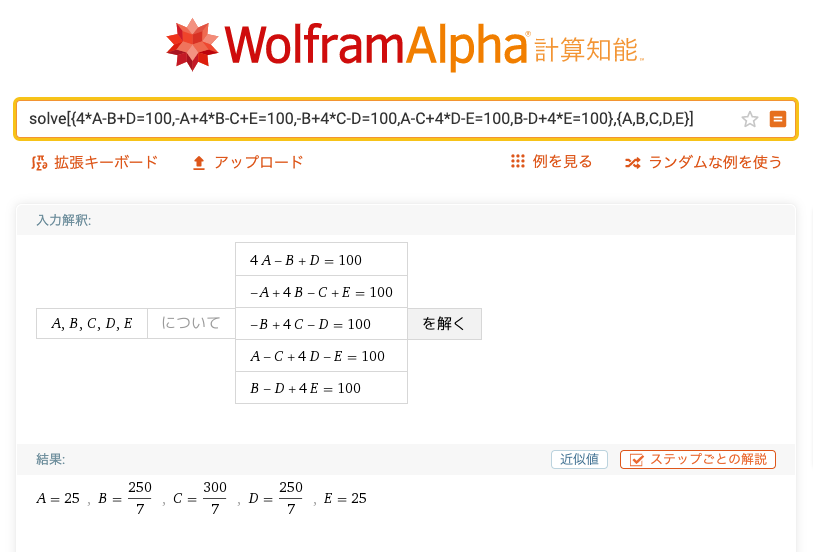
\includegraphics[width=15cm]{wolf.png}
	\caption{Solution of WalframAlpha~\cite{wolf}} 
\end{figure}

\begin{thebibliography}{99}
	\bibitem{wolf}WolframAlpha, \texttt{https://www.wolframalpha.com}, viewing date: Oct. 16th, 2019.
\end{thebibliography}


%
% END OF DOCUMENT
\end{document}
